% % % % % % % % %pART-16 % % % % % % %
\documentclass[12pt]{article}

\usepackage{pgfplots}
\pgfplotsset{chstyle/.style={xmin=-5, xmax=5, ymin=-5, ymax=5, xlabel=x, ylabel=y, axis lines=center, title=PGFPLOT tutorial, legend entries={$y=|x|$}} }

\author{Chandra Has\\ chandrahashbti@gmail.com}
\title{{\color{red}\bfseries Graphing} in \LaTeX\ using PGF/TikZ}\date{}

\begin{document}\maketitle\vskip-25pt\hrule\vskip10pt\centering

%\begin{tikzpicture}
%\begin{axis}[axis-options]
%\addplot[plot-options] formula;
%\end{axis}
%\end{tikzpicture}

%Plot formula:
%\addplot[plot-options] expression  {};
%\addplot[plot-options] coordinates {}; 
%\addplot[plot-options] table[table-options]       {};

%table-options
%x=colname, y=colname, x error= colname, y error=colname, col sep=comma (for csv file)

\begin{tikzpicture}
\begin{axis}[chstyle]
\addplot[red] {abs(x)};
\end{axis}
\end{tikzpicture}

\begin{tikzpicture}
\begin{axis}[xlabel=x, ylabel=y]
\addplot[red, mark=o] coordinates {(10,1) (90, 2) (100,3)};
\end{axis}
\end{tikzpicture}

\begin{tikzpicture}
\begin{semilogxaxis}[xlabel=x, ylabel=y]
\addplot[red, mark=o] coordinates {(10,1) (90, 2) (100,3)};
\end{semilogxaxis}
\end{tikzpicture}

\begin{tikzpicture}
\begin{axis}[xlabel=x, ylabel=y]
\addplot[red, mark=o] table[x=xdata, y=ydata] {
xdata	ydata
1	1
2	4
3	9
4	16
5	25
6	36
};
\end{axis}
\end{tikzpicture}

\begin{tikzpicture}
\begin{axis}[xlabel=x, ylabel=y]
\addplot[red, mark=o, error bars/.cd, y dir=both] table[x=xdata, y=ydata, y error=ybar] {
xdata	ydata	ybar
1	1	0.1
2	4	0.5
3	9	1.1
4	16	1.9
5	25	2.7
6	36	3.9

};
\end{axis}
\end{tikzpicture}


\begin{tikzpicture}
\begin{axis}[xlabel=x, ylabel=y]
\addplot[red, mark=o, error bars/.cd, y dir=both, y explicit] table[x=x, y=y, y error=ybar] {tabdata.txt};
\end{axis}
\end{tikzpicture}


\begin{tikzpicture}
\begin{axis}[xlabel=x, ylabel=y]
\addplot[red, mark=o, error bars/.cd, y dir=both, y explicit] table[x=x, y=y, y error=ybar, col sep=comma ] {tabdata.csv};
\end{axis}
\end{tikzpicture}

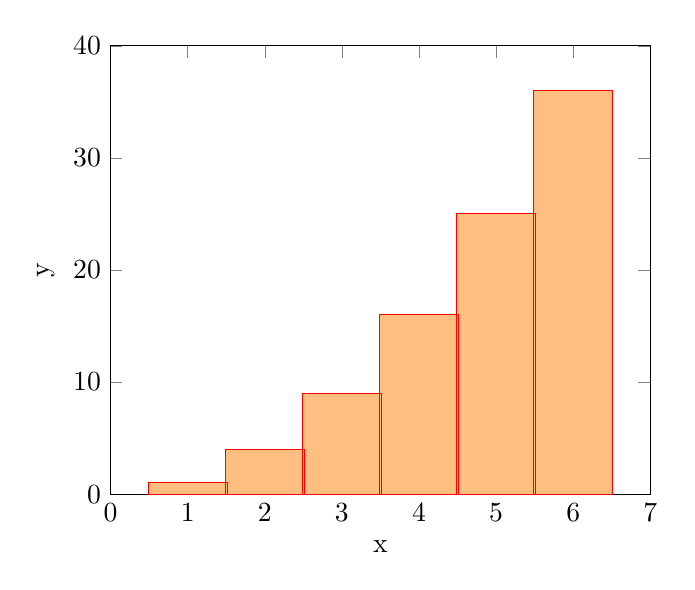
\begin{tikzpicture}
\begin{axis}[xlabel=x, ylabel=y, xmin=0, xmax=7, ymin=0, ymax=40]
\addplot[ybar, red, bar width=1cm, fill=orange!50] table[x=xdata, y=ydata] {
	xdata	ydata
	1	1
	2	4
	3	9
	4	16
	5	25
	6	36
};
\end{axis}
\end{tikzpicture}


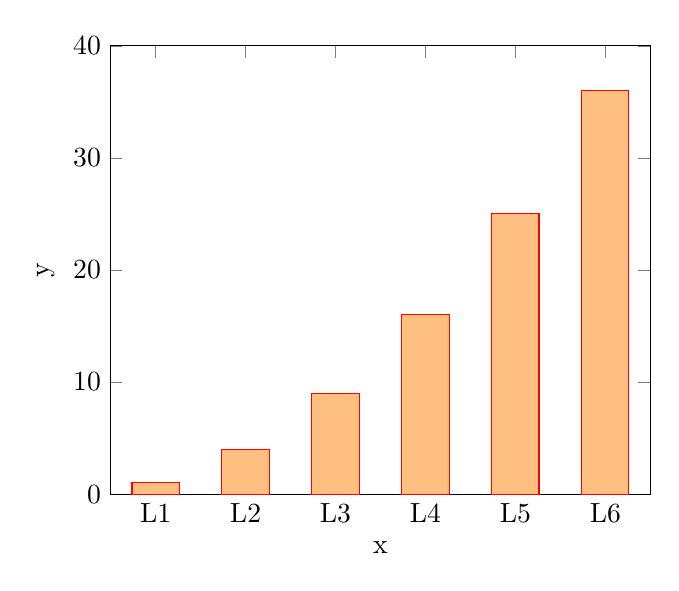
\begin{tikzpicture}
\begin{axis}[xlabel=x, ylabel=y, ymin=0, ymax=40, symbolic x coords = {L1, L2, L3, L4, L5, L6}]
\addplot[ybar, red, bar width=6mm, fill=orange!50] table[x=xdata, y=ydata] {
	xdata	ydata
	L1	1
	L2	4
	L3	9
	L4	16
	L5	25
	L6	36
};
\end{axis}
\end{tikzpicture}

\begin{tikzpicture}
\begin{axis}[xlabel=x, ylabel=y1, xmin=0, xmax=7, ymin=0, ymax=40, axis y line=left]
\addplot[red, mark=o, error bars/.cd, y dir=both, y explicit] table[x=x, y=y1, col sep=comma ] {double-y.csv};
\end{axis}

\begin{axis}[xlabel=x, ylabel=y2, xmin=0, xmax=7, ymin=0, ymax=7, axis y line=right, axis x line=none]
\addplot[red, mark=o, error bars/.cd, y dir=both, y explicit] table[x=x, y=y2, col sep=comma ] {double-y.csv};
\end{axis}
\end{tikzpicture}

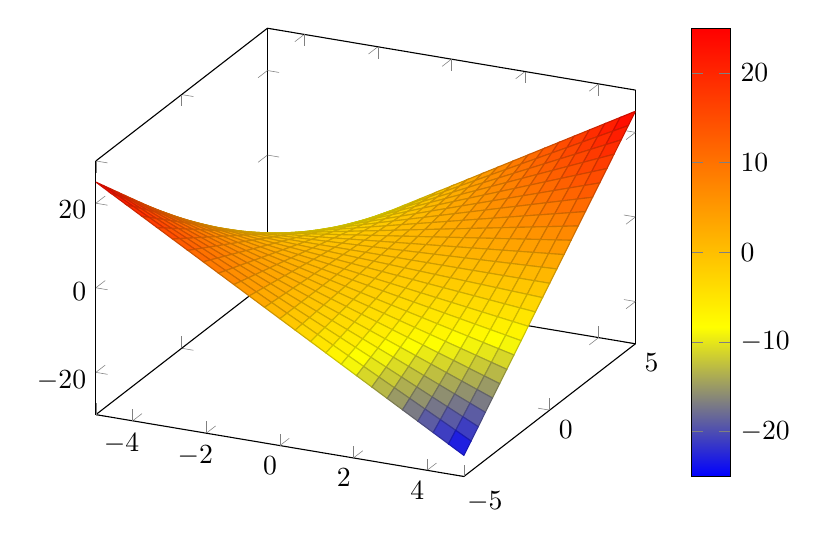
\begin{tikzpicture}
\begin{axis}[colorbar]
\addplot3[surf] {x*y};
\end{axis}
\end{tikzpicture}

\end{document}

